\section{Post-selection inferens}
Klassisk statistisk inferens kan ikke anvendes for adaptive procedurer.
I dette afsnit beskrives teste til inferens efter variabeludvælgelse med en adaptiv metode.
Teorien omkring post-selection inferens er udviklet i nyere tid og er stadig under udvikling.
R-pakkerne \texttt{covTest} og \texttt{selectiveInference} understøtter testene som beskrives i dette afsnit.

\subsection{Kovarians test} \label{subsec:kovarians_test}
I dette afsnit introduceres en test, der kan tildele \(p\)-værdier til prædiktorer som er udvalgt af adaptive procedurer.
Testen er baseret på LARS algoritmen og blev introduceret i \citep{lockhart}.

Betragt det velkendte lineær regression setup med en responsvariable \(\y \in \mathbb{R}^n\) og en matrix af prædiktorer \(\X \in \mathbb{R}^{n \times p}\), som er relateret ved
\begin{align}
\y = \X \beta + \boldsymbol{\epsilon}, \quad \boldsymbol{\epsilon} \sim N\del{\mathbf{0}, \sigma^2 \mathbf{I}}, \label{eq:set-up}
\end{align}
hvor \(\beta \in \mathbb{R}^p\) er ukendte koefficienter, som skal estimeres.

%For at motivere kovarians testen, vil vi først betragte forward-stepwise regression.
%Proceduren udvælger én prædiktor af gangen og vælger den prædiktor således at summen af kvadrerede residualer aftager mest.
%Lad \(\text{SSR}_k\) betegne summen af kvadrerede residualer for modellen med \(k\) prædiktorer.
%Da kan vi udlede en teststørrelse ved at betragte ændringen i SSR
%\begin{align*}
%R_k = \frac{1}{\sigma^2} \del{\text{SSR}_{k-1} - \text{SSR}_k},
%\end{align*}
%hvor \(\sigma\) antages at være kendt. 
%Denne teststørrelse følger en \(\chi_1^2\) fordeling.
%Hvis \(\sigma\) ikke er kendt, da den estimeres udfra sample variansen, hvilket resulterer i en \(F\)-test eller ækvivalent en \(t\)-test til at teste om variabel \(j\) er signifikant.
%
%Betragt forward stepwise regression: start med en tom model, tilføj en prædiktor af gangen, for hvert step vælg den prædiktor \(j\) som giver den største fald i SSR.
%Figur \ref{fig:covarians_test}(a) viser kvantilerne for \(R_1\) af forward stepwise regression imod en \(\chi_1^2\) fordeling, hvor \(\beta=0\).
%%
%\begin{figure}[H]
%\centering
% \scalebox{0.5}{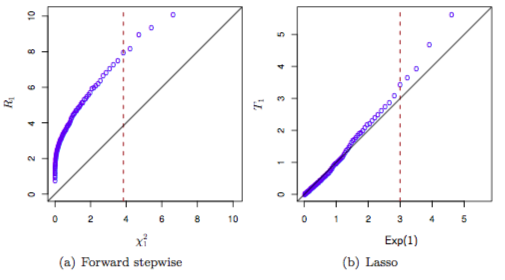
\includegraphics{fig/covarians_test.jpg}}
%\caption{Et .}
%\label{fig:covarians_test}
%\end{figure}
%%

Inden vi giver en formel beskrivelse af kovarians testen, gives en betingelse for model matricen \(\X\).
\begin{defn}[General position]
Kolonnerne \(\mathbf{X}_1, \ldots, \mathbf{X}_p\) siges at være i generel position hvis the affine span af enhver \(k+1\) vektorer \(s_1 \X_1, \ldots, s_{k+1} \X_{k+1}\) ikke indeholder ethvert element af mængden \(\cbr{\pm \X_i : \ i \neq i_1, \ldots, i_{k+1}}\) for ethvert fortegn \(s_1, \ldots, s_{k+1} \in \cbr{-1,1}\), for \(k < \min \cbr{n,p}\). 
\end{defn}
Ovenstående betingelse er svag og gælder blandt andet når indgangene af \(\X\) kommer af en kontinuert sandsynlighedsfordeling.
At kolonnerne af model matrix er i generel position sikrer at LARS og lasso stierne er entydig, som vises i \citep{lasso_unique}.

Herefter kan vi definere teststørrelsen af kovarians testen og forklare hvordan \(p\)-værdierne findes.
Vi antager det lineære regressions set-up i \eqref{eq:set-up} og at kolonner af \(\X\) er i generel position.
Vi ønsker, at teste om \(j\)'te prædiktor som er medtaget i den aktive mængde i \(\lambda_k\), dvs i \(k\)'te step af LARS algoritmen, er signifikant.
Lad \(\A_{k-1}\) betegne den aktive mængde i step \(k-1\) og lad \(\hat{\beta} \del{\lambda_{k+1}}\) være løsningen af lasso problemet i næste knot \(\lambda_{k+1}\).
Lad \(\tilde{\beta}_{\A_{k-1}} \del{\lambda_{k+1}}\) være løsningen af lasso problemet ved kun at anvende variablerne i \(\A_{k-1}\)
\begin{align*}
\tilde{\beta}_{\A_{k-1}} \del{\lambda_{k+1}} = \argmin_{\beta_{\A_{k-1}} \in \R^{\vert \A_{k-1} \vert}} \frac{1}{2n} \left\Vert \y - \X_{\A_{k-1}} \beta_{\A_{k-1}} \right\Vert_2^2 + \lambda_{k+1} \left\Vert \beta_{\A_{k-1}} \right\Vert_1,
\end{align*}
hvor \(\X_{\A_{k-1}}\) består af kolonnerne af \(\X\), som svarer til prædiktorerne i \(\A_{k-1}\).
Da kan vi definere kovarians testen
\begin{align}
T_k^\text{cov} = \frac{1}{\sigma^2} \del{ \left\langle \y, \X \hat{\beta} \del{\lambda_{k+1}} \right\rangle - \left\langle  \y, \X_{\A_{k-1}} \tilde{\beta}_{\mathcal{A}_{k-1}} \del{\lambda_{k+1}} \right\rangle}. \label{eq:6.5}
\end{align}
Intuitivt, er teststørrelsen af kovarians testen i \eqref{eq:6.5} en funktion af differensen mellem \(\X \hat{\beta}\) og \(\X_{\A_{k-1}} \tilde{\beta}_{\A_{k-1}}\), dvs de fittede værdier givet ved at medtage \(j\)'te prædiktor i den nuværende aktive mængde og undlade den.
Kovarians teststørrelsen evalueres i næste knot \(\lambda_{k+1}\), da \(j\)'te koefficient stadig er lig nul i \(\lambda_k\) og derfor
\begin{align*}
\X \hat{\beta} \del{\lambda_k} = \X_{\A_{k-1}} \hat{\beta}_{\A_{k-1}} \del{\lambda_k} = \X_{\A_{k-1}} \tilde{\beta}_{\A_{k-1}} \del{\lambda_k}
\end{align*}
Det naturlig valg for tuning parameteren i \eqref{eq:6.5} er derfor \(\lambda= \lambda_{k+1}\).
Navnet af testen kommer af at tælleren i \eqref{eq:6.5} kan skrives som differensen mellem empiriske kovarianser og et lille led.
Desto større kovarians af \(\y\) og \(\X \hat{\beta}\) sammenlignet med \(\X_{\A_{k-1}} \hat{\beta}_{A_{k-1}}\), desto vigtigere er \(j\)'te prædiktor i modellen \(\A \cup \cbr{j}\).

Under nulhypotesen at den nuværende lasso model indeholder alle sande aktive variable, som skal skrives \(\mathcal{A}_{k-1} \supseteq \text{supp} \del{\beta^*}\), hvor \(\beta^*\) er den sande koefficient vektor, da har teststørrelsen i \eqref{eq:6.5} en asymptotisk standard eksponential fordeling
\begin{align*}
T_k^\text{cov} \overset{d}{\rightarrow} \text{Exp}\del{1}.
\end{align*}
Hvis \(\sigma^2\) er ukendt, kan den estimeres under den fulde model \(\hat{\sigma}^2 = \frac{1}{n-p} \text{SSR}_p\). 
Dette indsættes i \eqref{eq:6.5}, og eksponential testen bliver en eksakt \(F_{2,n-p}\) test.

Denne test er også det naturlige analog til degrees of freedom resultaterne for lasso \eqref{eq:df_lasso} og LARS (section 2.5).
Lasso med \(k\) ikke-nul koefficienter forventes at have \(k\) frihedsgrader, og LARS anvender en frihedsgrad for hver segment \(\del{\lambda_{k+1}, \lambda_k}\) langs stien.
Kovarians testen har middelværdi lig en, som er antal frihedsgrader per trin.
%
Hernæst vil vi introducere en alternativ form af teststørrelsen i \eqref{eq:6.5}, som er nyttigt af beregningsmæssige årsager.
\begin{align*}
T_k^\text{cov} = \frac{1}{\sigma^2} \omega_k^2 \cdot \lambda_k \del{\lambda_k - \lambda_{k+1}},
\end{align*}
hvor \(\lambda_k\) og \(\lambda_{k+1}\) er LARS knots i step \(k\) og \(k+1\) af stien og \(\omega_k\) er vægten givet i \eqref{eq:post_42}.


%
%Hvis \(\X\) er ortogonal, da er teststørrelsen for kovarians testen givet ved
%\begin{align*}
%T_k^\text{cov} = \frac{1}{\sigma^2} \lambda_k \del{\lambda_k - \lambda_{k+1}}
%\end{align*} 
%Derudover fandt vi at \eqref{eq:ortogonal_lasso} som også kan skrives \(\hat{\beta}_j = S_\lambda \del{\frac{1}{n} \mathbf{x}_j^T \y}\).
%Lad \(\mathbf{U}_j = \mathbf{x}_j^T \y\) for \(j=1,\ldots, p\). 
%Knots i lasso stien er blot værdierne af \(\lambda\) for hvilket koefficienterne er ikke-nul
%\begin{align*}
%\lambda_1 = \vert \mathbf{U}_{(1)} \vert, \quad \lambda_2 = \vert \mathbf{U}_{(2)} \vert, \quad \ldots, \lambda_p = \vert \mathbf{U}_{(p)} \vert, \quad,
%\end{align*}
%hvor \(\vert \mathbf{U}_{(1)} \vert \geq \vert \mathbf{U}_{(2)} \vert \geq \dots \geq \vert \mathbf{U}_{(p)} \vert\) er order statistics af \(\vert \mathbf{U}_1 \vert, \ldots, \vert \mathbf{U}_p \vert\).
%Derfor 
%\begin{align*}
%T_k^\text{cov} = \frac{1}{\sigma^2}  \vert \mathbf{U}_{(k)} \vert \del{ \vert \mathbf{U}_{(k)} \vert -  \vert \mathbf{U}_{(k+1)} \vert}
%\end{align*}


Kovarians testen har nogle begrænsninger.
Først skal der gælde en betingelse for model matricen \(\X\).
Hvis der eksisterer en kategorisk variabel blandt prædiktorerne, og den resulterende variabel beskrives af dummy variable, da er antagelse om at kolonnerne af \(\X\) er i general position altså ikke overholdt.
Derudover tager testen ikke højde for, hvis nogle variable medtages i modellen mere end én gang (som er tilladt for lasso modificeringen af LARS algoritmen), da behandles hver situation separat og testene udføres separat.
Til sidst er testen kun asymptotisk.

I næste afsnit introduceres en test som kan anvendes efter modeludvælgelse og som giver en eksakt fordeling af teststørrelsen.

\subsection{Teste baseret på polyhedral lemmaet}
I dette afsnit introduceres \textit{TG testen}, hvor TG står for "truncated gaussian" som er baseret på polyhedral lemmaet. 
Afsnit er baseret på \citep{post_inference}.

Indledningsvis introduceres notation som anvendes i dette afsnit.
For en matrix \(M \in \R^{n \times p}\) og liste \(S = \sbr{s_1, \ldots, s_r} \subseteq \sbr{1, \ldots, p}\), skriver vi \(M_S \in \R^{n \times \vert S \vert}\) for submatricen som findes ved at udtrække tilhørende kolonner af \(M\).
Tilsvarende for en vektor \(x \in \R^p\), betegnes \(x_S\) for subvektoren.
Vi skriver \(\del{M^T M}^+\) for Moore Penrose pseudoinverse af den kvadratiske matrix \(M\) og \(M^+ = \del{M^T M}^+ M^T\) for pseudoinverse af en rektangulær matrix \(M\).
Vi anvender \(P_L\) for projektions operatoren på det lineære underrum \(L\).
\(\mathbb{P}_{\teta^T \tmu = 0} \del{\cdot \given y \in \mathcal{P}} \) er sandsynligheds målet under \(\tmu\) for hvilket \(\teta^T \tmu =0 \) betinget \(\y \in \mathcal{P}\). 

Antag \(\y \sim N(\tmu, \Sigma)\), hvor \(\tmu \in \R^{n}\) er ukendt, men \(\Sigma \in \R^{n \times n}\) er kendt.
Dette generaliserer vores setup i \eqref{eq:set-up}.
Vi betragter polyhedronen \(\mathcal{P} = \cbr{\y : \ \Gamma \y \geq u}\), hvor \(\Gamma \in \mathbb{R}^{m \times n}\) og \(u \in \mathbb{R}^m\) er faste og uligheden skal fortolkes elementvis.
For et fast \(\teta \in \R^n\) ønsker vi at lave inferens af \(\teta^T \tmu\) betinget \(\y \in \mathcal{P}\).
Nedenfor gives en alternativ repræsentation af \(\mathcal{P}\).



%Antag \(\y \sim N\del{\boldsymbol{\mu}, \sigma^2 \mathbf{I}_{n \times n}}\) og at vi ønsker at lave inferens betinget på hændelsen \(\cbr{\mathbf{A} \y \leq b}\).
%Mere præcis ønsker vi at lave inferens om \(\boldsymbol{\eta}^T \boldsymbol{\mu}\), hvor \(\boldsymbol{\eta}\) muligvis afhænger af udvægelsen.
%Hvis lasso, LARS .. har udvalgt denne mængde, da kan vi udføre inferens  af de udvalgte variable.
%Vi kunne eventuelt være interesseret i regressions koefficienterne af \(\y\) på \(\X_\mathcal{A}\), dvs \(\hat{\theta}= \del{\X_\mathcal{A}^T \X_\mathcal{A}}^{-1} \X_\mathcal{A}^T \y\).
%Disse svarer til populations parametrene \(\theta= \del{\X_\mathcal{A}^T \X_\mathcal{A}}^{-1} \X_\mathcal{A}^T \boldsymbol{\mu}\), koefficienterne af projectionen af \(\boldsymbol{\mu}\) på \(\X_\mathcal{A}\).
%Dermed kunne \(\boldsymbol{\eta}^T \boldsymbol{\mu}\) svarer til én af disse koefficienter, og dermed er \(\boldsymbol{\eta}\) en af kolonnerne af \(\X_\mathcal{A} \del{\X_\mathcal{A}^T \X_\mathcal{A}}^{-1}\). Dette eksempel fortsættes senere.

%\subsubsection{Conditioning on a single polyhedron}
%Antag \(\y \sim N \del{\boldsymbol{\mu}, \Sigma}\) og \(\boldsymbol{\eta} \in \mathbb{R}^n\) er en potential retning.
%For at forstå fordelingen af
%\begin{align*}
%\boldsymbol{\eta}^T \y \given \cbr{ \mathbf{A} \y \leq b},
%\end{align*}
%kan vi omskrive \(\cbr{\mathbf{A} \y \leq b}\) udfra \(\boldsymbol{\eta}^T \y\) og en komponent \(\mathbf{z}\) som er uafhængig af \(\boldsymbol{\eta}^T \y\). Denne komponent er givet ved
%\begin{align}
%\mathbf{z} = \del{\mathbf{I} - \mathbf{c} \boldsymbol{\eta}^T} \y, \label{eq:z}
%\end{align}
%hvor 
%\begin{align}
%\mathbf{c} = \Sigma \boldsymbol{\eta} \del{\boldsymbol{\eta}^T \Sigma \boldsymbol{\eta}}^{-1}. \label{eq:c}
%\end{align}
%Det ses let, at \(\mathbf{z}\) er ukorreleret og dermed uafhængig af \(\boldsymbol{\eta}^T \y\).
%Hvis \(\Sigma = \sigma^2 \mathbf{I}\), da er \(\mathbf{z}\) blot residualen \(\del{\mathbf{I} - P_{\boldsymbol{\eta}}} \y \) fra projektionen \(\y\) på \(\boldsymbol{\eta}\).
%Vi kan nu omskrive \(\cbr{\mathbf{A} \y \leq b}\) udfra \(\boldsymbol{\eta}^T \y\) og \(\mathbf{z}\).
%
\begin{lem}[Polyhedral lemma] \label{lem:polyhedral}
%Lad \(\mathbf{z}\) være defineret som i \eqref{eq:z} og \(\mathbf{c}\) som i \eqref{eq:c}. 
For ethvert \(\Sigma\) og \(\teta\) således at \(\teta^T \Sigma \teta \neq 0\), da gælder, at
\begin{align}
\Gamma \y \geq u \ \Longleftrightarrow \ \mathcal{V}^- \del{\y} \leq \boldsymbol{\eta}^T \y \leq \mathcal{V}^+ \del{\y}, \  \mathcal{V}^0 \del{\y} \leq 0, \label{eq:post_8}
\end{align}
hvor
\begin{align}
\mathcal{V}^- \del{\y} &= \max_{j: \rho_j > 0} \frac{u_j - \del{\Gamma \y}_j + \rho_j \boldsymbol{\eta}^T \y}{\rho_j}, \label{eq:V-} \\
\mathcal{V}^+ \del{\y} &= \min_{j: \rho_j < 0} \frac{u_j - \del{\Gamma \y}_j + \rho_j \boldsymbol{\eta}^T \y}{\rho_j}, \label{eq:V+} \\
\mathcal{V}^0 \del{\y} &= \max_{j: \rho_j = 0} \del{u_j - \del{\Gamma \y}_j}, \label{eq:V0} 
\end{align}
og \(\rho=\frac{\Gamma \Sigma \boldsymbol{\eta}}{\teta^T \Sigma \teta}\).
Yderligere  er \(\boldsymbol{\eta}^T \y\) og \(\del{\mathcal{V}^-\del{\y}, \mathcal{V}^+\del{\y},\mathcal{V}^0\del{\y}}\) uafhængige. 
\end{lem}
%\begin{proof}
%Vi kan dekomponere \(\y = \mathbf{c} \del{\boldsymbol{\eta}^T \y} + \mathbf{z}\) og opskrive polyhedronet som følgende
%\begin{align*}
%\cbr{\mathbf{A} \y \leq b} &= \cbr{\mathbf{A} \del{\mathbf{c} \del{\boldsymbol{\eta}^T \y} + \mathbf{z}} \leq b} \\
%&= \cbr{\mathbf{A} \mathbf{c} \del{\boldsymbol{\eta}^T \y} \leq b - \mathbf{A} \mathbf{z} } \\
%&= \cbr{\del{\mathbf{A} \mathbf{c}}_j \del{\boldsymbol{\eta}^T \y} \leq b_j - \del{\mathbf{A} \mathbf{z}}_j \text{ for alle } j} \\
%&= \begin{cases}
%\boldsymbol{\eta}^T \y \leq \frac{b_j - \del{\mathbf{A} \mathbf{z}}_j}{\del{\mathbf{A} \mathbf{c}}_j}, \quad j:\del{\mathbf{A} \mathbf{c}}_j > 0 \\
%\boldsymbol{\eta}^T \y \geq \frac{b_j - \del{\mathbf{A} \mathbf{z}}_j}{\del{\mathbf{A} \mathbf{c}}_j}, \quad j:\del{\mathbf{A} \mathbf{c}}_j < 0 \\
%0 \leq b_j - \del{\mathbf{A} \mathbf{z}}_j, \quad j:\del{\mathbf{A} \mathbf{c}}_j = 0
%\end{cases}.
%\end{align*}
%Da \(\boldsymbol{\eta}^T \y \) er den samme mængde for alle \(j\), må det mindste være maksimum af de nedre grænser, som er \(\mathcal{V}^- \del{\mathbf{z}}\), og ikke mere end minimum af de øvre grænser, som er \(\mathcal{V}^+ \del{\mathbf{z}}\).
%\end{proof}
Resultatet i \eqref{eq:post_8} hvor \(\mathcal{V}^-\), \(\mathcal{V}^+\) og \(\mathcal{V}^0\) defineres i \eqref{eq:V-}-\eqref{eq:V0} er deterministisk og gælder for alle \(\y\).
Blot uafhængighedsresultatet afhænger af normaliteten af \(\y\).
Se figur \ref{fig:polyhedron} for en geometrisk illustration af lemmaet.
Intuitivt kan resultatet forklares som følgende, hvor vi antager, at \(\Sigma= \mathbf{I}\).
Først dekomponeres \(\y=P_{\boldsymbol{\eta}} \y + P_{\boldsymbol{\eta}^\perp} \y\), hvor \(P_{\boldsymbol{\eta}} \y = \frac{\boldsymbol{\eta} \boldsymbol{\eta}^T \y}{\Vert \boldsymbol{\eta} \Vert_2^2}\) er projektionen af \(\y\) langs \(\boldsymbol{\eta}\) og  \(P_{\boldsymbol{\eta}^\perp} \y = \y - P_{\boldsymbol{\eta}} \y\) er projektionen på ortokomplementet af \(\boldsymbol{\eta}\).
Vi kan betragte \(\y\) som en afvigelse fra \(P_{\boldsymbol{\eta}^\perp} \y\) af en mængde \(\boldsymbol{\eta}^T \y\), langs linjen bestemt af \(\boldsymbol{\eta}\).
Mængderne \(\mathcal{V}^-\) og \(\mathcal{V}^+\) betegner hvor langt vi kan afvige fra hver side af \(P_{\boldsymbol{\eta}^\perp} \y\) inden \(\y\) forlader polyhedronen.
Dette giver anledning til uligheden \(\mathcal{V}^- \leq \boldsymbol{\eta}^T \y \leq \mathcal{V}^+\).
Nogle flader af polyhedronen kan være perfekt justeret med \(\boldsymbol{\eta}\), dvs deres normal vektorer kan være ortogonale med \(\boldsymbol{\eta}\).
Dette kan tjekkes udfra \(\mathcal{V}^0\) ved at \(\y\) ligger på den rigtige side af disse flader.  
%--
%Betinget \(P_{\boldsymbol{\eta}^\perp} \y\), ses at hændelsen \(\cbr{\mathbf{A} \y \leq b}\) er ækvivalent med hændelsen \(\mathcal{V}^- \del{\y} \leq \boldsymbol{\eta}^T \y \leq \mathcal{V}^+ \del{\y}\). Yderligere er \(\mathcal{V}^- \del{\y}\) og \(\mathcal{V}^+ \del{\y}\) uafhængige af \(\boldsymbol{\eta}^T \y\), da disse kun er funktioner af \(P_{\boldsymbol{\eta}^\perp} \y\), som er uafhængige af \(\y\).
%--

%
\begin{figure}[H]
\centering
\scalebox{1}{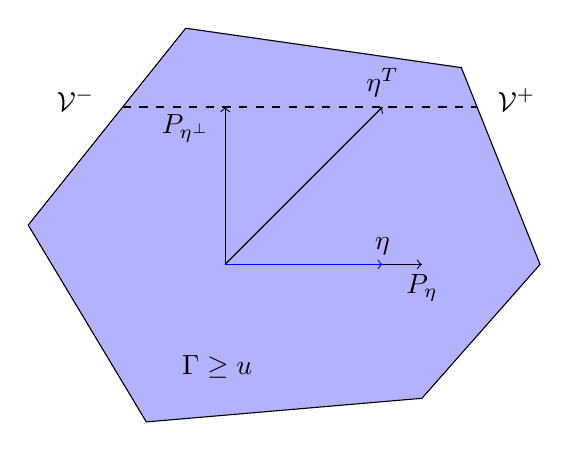
\begin{tikzpicture}
\draw (-1,-2) -- (-2.5,0.5) -- (-0.5,3)-- (3,2.5) -- (4,0) -- (2.5,-1.7) -- (-1,-2)[fill = blue!30];
\draw [<-] (0,2) node [label={[xshift=-0.5cm, yshift=-0.7cm]$P_{\boldsymbol{\eta}^\perp} \y$}] {} -- (0,0);
\draw[<-] (2.5,0) node [below] {$P_{\boldsymbol{\eta}} \y$} -- (0,0);
\draw[<-][blue] (2,0) node [black, above] {$\boldsymbol{\eta}$} -- (0,0);
\draw[<-] (2,2) node [above] {$\boldsymbol{\eta}^T \y$} -- (0,0) node [label={[xshift=1.7cm, yshift=1cm]$\y$}] {};
\draw[dashed] (-1.3,2) node [label={[xshift=-0.6cm, yshift=-0.3cm]$\mathcal{V}^- \del{\y}$}] {} -- (3.2,2) node [label={[xshift=0.5cm, yshift=-0.3cm]$\mathcal{V}^+ \del{\y}$}] {};
\draw node [label={[xshift=-0.1cm, yshift=-1.7cm]$\cbr{\Gamma \y \geq u}$}] {};
\end{tikzpicture}}
\caption{Geometri af polyhedron udvælgelsen som trunkering. For simplicitet antages at \(\Sigma = \mathbf{I}\). Det blå område er polyhedron mængden \(\cbr{\y : \ \Gamma \y \geq u}\).
Ved at opdele \(\y\) til dens projektion på \(\teta\) og dens projektion på det ortogonale komplement af \(\teta\), ses at \(\Gamma \y \geq u\) er opfyldt, hvis og kun hvis \(\teta^T \y\) ikke afviger for langt fra \(P_{\boldsymbol{\eta}^\perp} \y\), dvs den skal fastholdes imellem grænserne \(\mathcal{V}^-\) og \(\mathcal{V}^+\).
Yderligere er grænserne \(\mathcal{V}^-\) og \(\mathcal{V}^+\) kun funktioner af \(P_{\boldsymbol{\eta}^\perp} \y\), derfor er de uafhængige af \(\teta^T \y\) under normalitet.} \label{fig:polyhedron}
\end{figure}
%

Af lemma \ref{lem:polyhedral} kan fordelingen af enhver lineær funktion \(\boldsymbol{\eta}^T \y\) betinget \(\Gamma \y \geq u\) skrives som følgende betinget fordeling
\begin{align*}
\boldsymbol{\eta}^T \y \given \mathcal{V}^- \del{\y} \leq \boldsymbol{\eta}^T \y \leq \mathcal{V}^+ \del{\y}, \ \mathcal{V}^0 \del{\y} \leq 0.
\end{align*}
Da \(\boldsymbol{\eta}^T \y\) er normalfordelt, er overstående trunkeret normalfordelt.
En simpel transformation fører til pivotal statistic, som er kritisk for inferens af \(\boldsymbol{\eta}^T \tmu\).

\begin{lem}  \label{lem:lem2}
Lad \(\Phi \del{x}\) betegne fordelingsfunktionen af en standard normalfordeling, da er fordelingsfunktionen for en normalfordeling med middelværdi \(\mu\) og varians \(\sigma^2\) af en stokastisk variable indenfor intervallet \(\sbr{a,b}\) givet ved
\begin{align*}
F_{\mu, \sigma^2}^{\sbr{a,b}} \del{x} = \frac{\Phi\del{\frac{x-\mu}{\sigma}} - \Phi\del{\frac{a-\mu}{\sigma}}}{\Phi\del{\frac{b-\mu}{\sigma}} - \Phi\del{\frac{a-\mu}{\sigma}}}.
\end{align*}
For \(\boldsymbol{\eta}^T \Sigma \boldsymbol{\eta} \neq 0\), da følger teststørrelsen \(F_{\boldsymbol{\eta}^T \tmu, \boldsymbol{\eta}^T \Sigma \boldsymbol{\eta}}^{\sbr{\mathcal{V}^-,\mathcal{V}^+}} \del{\boldsymbol{\eta}^T \y} \) betinget \(\Gamma \y \geq u\) en standard uniform fordeling. Dvs
\begin{align*}
\mathbb{P} \del{F_{\boldsymbol{\eta}^T \tmu, \boldsymbol{\eta}^T \Sigma \boldsymbol{\eta}}^{\sbr{\mathcal{V}^-,\mathcal{V}^+}} \del{\boldsymbol{\eta}^T \y} \leq \alpha \given \Gamma \y \geq u} = \alpha, 
\end{align*}
for ethvert \(0 \leq \alpha \leq 1\), hvor \(\mathcal{V}^-\) og \(\mathcal{V}^+\) er defineret i \eqref{eq:V-} samt \eqref{eq:V+}. 
\end{lem}
%
Denne pivotal statistic i lemmaet fører til gyldige betinget \(p\)-værdier for at teste nulhypotesen \(H_0: \boldsymbol{\eta}^T \boldsymbol{\mu}=0\) og tilhørende betinget konfidensintervaller for \(\boldsymbol{\eta}^T \tmu\).
Herefter betragtes one-sided inferens efterfulgt af two-sided inferens.
%
\begin{lem} \label{lem:lem3}
Givet \(\boldsymbol{\eta}^T \Sigma \boldsymbol{\eta} \neq 0\), antag at vi vil teste
\begin{align*}
H_0: \boldsymbol{\eta}^T \tmu=0 \quad \text{imod} \quad H_1: \boldsymbol{\eta}^T \tmu > 0.
\end{align*}
Definer teststørrelsen
\begin{align}
T=1- F_{0, \boldsymbol{\eta}^T \Sigma \boldsymbol{\eta}}^{\sbr{\mathcal{V}^-, \mathcal{V}^+}} \del{\boldsymbol{\eta}^T \y}, \label{eq:post_1.14}
\end{align}
hvor fordelingsfunktionen af \(\boldsymbol{\eta}^T \y \sim N \del{0,  \boldsymbol{\eta}^T \Sigma \boldsymbol{\eta}}\) i intervallet \(\sbr{\mathcal{V}^-, \mathcal{V}^+}\) er givet i lemma \ref{lem:lem2}.
Da er \(T\) en gyldig \(p\)-værdi for \(H_0\) betinget \(\Gamma \y \geq u\)
\begin{align}
\mathbb{P}_{\boldsymbol{\eta}^T \tmu=0} \del{T \leq \alpha \given \Gamma \y \geq u} = \alpha, \label{eq:post_1.15}
\end{align}
for ethvert \(0 \leq \alpha \leq 1\). 
Definer \(\delta_{\alpha}\) som opfylder, at
\begin{align*}
1-F_{\delta_{\alpha}, \boldsymbol{\eta}^T \Sigma \boldsymbol{\eta}}^{\sbr{\mathcal{V}^- \mathcal{V}^+}} \del{\boldsymbol{\eta}^T \y} &= \alpha.
\end{align*}
Da er \(I= [\delta_\alpha, \infty )\) et gyldig one-sided konfidensinterval for \(\teta^T \tmu\) betinget \(\Gamma \y \geq u\)
\begin{align*}
\mathbb{P} \del{\boldsymbol{\eta}^T \tmu \geq \delta_\alpha \given \Gamma \y \geq u} = 1- \alpha.
\end{align*}
\end{lem}
%
Bemærk-----
Herefter betragtes two-sided inferens.
%
\begin{lem} \label{lem:lem4}
Givet \(\boldsymbol{\eta}^T \Sigma \boldsymbol{\eta} \neq 0\), antag at vi vil teste
\begin{align*}
H_0: \boldsymbol{\eta}^T \tmu=0 \quad \text{imod} \quad H_1: \boldsymbol{\eta}^T \tmu \neq 0.
\end{align*}
Definer teststørrelsen
\begin{align}
T=2 \cdot \min\cbr{F_{0, \boldsymbol{\eta}^T \Sigma \boldsymbol{\eta}}^{\sbr{\mathcal{V}^-, \mathcal{V}^+}} \del{\boldsymbol{\eta}^T \y}, 1 - F_{0, \boldsymbol{\eta}^T \Sigma \boldsymbol{\eta}}^{\sbr{\mathcal{V}^-, \mathcal{V}^+}} \del{\boldsymbol{\eta}^T \y}}, \label{eq:post_1.18}
\end{align}
hvor fordelingsfunktionen af \(\boldsymbol{\eta}^T \y \sim N \del{0,  \boldsymbol{\eta}^T \Sigma \boldsymbol{\eta}}\) i intervallet \(\sbr{\mathcal{V}^-, \mathcal{V}^+}\) er givet i lemma \ref{lem:lem2}.
Da er \(T\) en gyldig \(p\)-værdi for \(H_0\) betinget \(\Gamma \y \geq u\)
\begin{align}
\mathbb{P}_{\boldsymbol{\eta}^T \tmu=0} \del{T \leq \alpha \given \Gamma \y \geq u} = \alpha, \label{eq:post_1.19}
\end{align}
for ethvert \(0 \leq \alpha \leq 1\). 
Definer \(\delta_{\frac{\alpha}{2}}, \delta_{1-\frac{\alpha}{2}}\) som opfylder, at
\begin{align}
1-F_{\delta_{\frac{\alpha}{2}}, \boldsymbol{\eta}^T \Sigma \boldsymbol{\eta}}^{\sbr{\mathcal{V}^- \mathcal{V}^+}} \del{\boldsymbol{\eta}^T \y} &= \frac{\alpha}{2}, \label{eq:post_20} \\
1-F_{\delta_{1-\frac{\alpha}{2}}, \boldsymbol{\eta}^T \Sigma \boldsymbol{\eta} }^{\sbr{\mathcal{V}^- \mathcal{V}^+}} \del{\boldsymbol{\eta}^T \y} &= 1-\frac{\alpha}{2}. \label{eq:post_21}
\end{align}
Da gælder, at
\begin{align}
\mathbb{P} \del{\delta_{\frac{\alpha}{2}} \leq  \boldsymbol{\eta}^T \tmu \leq \delta_{1-\frac{\alpha}{2}} \given \Gamma \y \geq u} = 1- \alpha. \label{eq:post_22}
\end{align}
\end{lem}
%
Teststørrelsen i \eqref{eq:post_1.18} defineret som minimum af den trunkerede fordelingsfunktion af normalfordelingen og overlevelsesfunktionen, har magt imod den alternative hypotese \(H_1: \boldsymbol{\eta}^T \tmu \neq 0\).
Beviset for dens nulhypotese i \eqref{eq:post_1.19} kommer af, at hvis \(U\) følger en standard uniform fordelingen, da gør \(2 \cdot \min \cbr{U,1-U}\) også.
Konstruktionen af konfidensintervallet i \eqref{eq:post_20}, \eqref{eq:post_21} og \eqref{eq:post_22} anvendes igen monotonicitet af en trunkeret normal overlevelsesfunktion i den underliggende middelværdi parameter.


Herefter vil vi vise at modeludvælgelses hændelsen for LARS og lasso kan karakteriseres som et polyhedron (dvs kegler) på formen \(\cbr{\y : \ \Gamma \y \geq u}\).
\subsubsection{Polyhedral mængder for LARS udvælgelses hændelse}
Lad os opsummere en kort beskrivelse af stepsene i LARS algoritmen.
I step \(k=1\), initialiseres mængden af aktive variable og listen af fortegn med \(\A=\sbr{j_1}\) og \(s_{\A_1} = \sbr{s_1}\), hvor \(j_1\) og \(s_1\) opfylder
\begin{align}
\del{j_1, s_1} = \argmax_{j=1,\ldots, p, \ s \in \sbr{-1,1}} s \X_j^T \y. \label{eq:polyhedron_rep_LARS1}
\end{align}
Første knot er givet ved
\begin{align*}
\lambda_1 = s_1 \X_{j_1}^T \y.
\end{align*}
For det generelle step \(k > 1\), konstrueres listen \(\A_k\) ved at tilføje \(j_k\) til \(\A_{k-1}\) og \(s_{\A_k}\) konstrueres ved at tilføje \(s_k\) til \(s_{\A_{k-1}}\), hvor \(j_k\) og \(s_k\) opfylder, at
\begin{align}
\del{j_k, s_k} = \argmax_{j \notin \A_{k-1} , \ s \in \sbr{-1,1}} \frac{\X_j^T P_{\A_{k-1}}^\perp \y}{s - \X_j^T \del{\X_{\A_{k-1}}^+}^T s_{\A_{k-1}}} \cdot \mathbb{1} \cbr{\frac{\X_j^T P_{\A_{k-1}}^\perp \y}{s - \X_j^T \del{\X_{\A_{k-1}}^+}^T s_{\A_{k-1}}} \leq \lambda_{k-1}}, \label{eq:polyhedron_rep_LARS2}
\end{align}
hvor \(P_{\A_{k-1}}^\perp \) er projektionen ortogonal med column space af \(\X_{\A_{k-1}}\), \(\mathbb{1} \cbr{\cdot}\) er indikator funktionen og \(\lambda_{k-1}\) er knot værdien af step \(k-1\).
Det \(k\)'te knot er da givet ved
\begin{align}
\lambda_k = \frac{\X_{j_k}^T P_{\A_{k-1}}^\perp \y}{s_k - \X_{j_k}^T \del{\X_{\A_{k-1}}^+}^T s_{\A_{k-1}}}. \label{eq:polyhedron_rap_LARS3}
\end{align}
Algoritmen afsluttes efter \(k\)-step hvis \(k=p\) eller hvis \(\lambda_{k+1} < 0\).

Herefter vil vi verificere at LARS udvælgelses hændelsen
\begin{align}
\mathcal{P} = \cbr{y: \ \hat{\A}_k \del{\y} = \A_k, \ \hat{s}_{\A_k} \del{\y} = s_{\A_k}, \ \hat{S}_\ell \del{\y} = S_\ell, \ \ell = 1, \ldots, k} \label{eq:post_28}
\end{align}
er en polyhedron på formen \(\mathcal{P} = \cbr{\y : \ \Gamma \y \geq 0}\).

Polyhedral repræsentationen for \(\mathcal{P}\) i \eqref{eq:post_28} kan bevises vha induktion.
For \(k=1\), finder vi, udfra \eqref{eq:polyhedron_rep_LARS1} at
\begin{align*}
c \del{j_1, s_1}^T \y \geq c \del{j,s}^T \y, \ \forall j \neq j_1, \ s \in \cbr{-1,1},
\end{align*}
hvor \(c \del{j,s} = s \X_j\).
Hermed finder vi, at \(\Gamma\) har \(2 \del{p-1}\) rækker, som er givet ved \(c \del{j_1, s_1} - c \del{j, s}\) for \(j \neq j_1, \ s \in \cbr{-1,1}\).
For \(k-1\) step kan optimaliteten af \(j_k\) og \(s_k\) i \eqref{eq:polyhedron_rep_LARS2} udtrykkes som
\begin{align*}
c \del{j_k, s_k, \A_{k-1}, s_{\A_{k-1}}}^T \y &\geq c \del{j, s, \A_{k-1}, s_{\A_{k-1}}}^T \y, \ \forall \del{j,s} \in S_k \backslash \cbr{\del{j_k, s_k}}, \\
c \del{j_k, s_k, \A_{k-1}, s_{\A_{k-1}}}^T \y &\geq 0,
\end{align*}
hvor \(c \del{j, s, \A_{k-1}, s_{\A_{k-1}}} = \frac{P_{\A_{k-1}}^\perp \X_j}{s - \X_j^T \del{\X_{\A_{k-1}}^+}^T s_{\A_{k-1}}}\).
Mængden \(S_k\) er karakteriseret ved
\begin{align*}
c \del{j, s, \A_{k-1}, s_{\A_{k-1}}}^T \y &\leq \lambda_{k-1}, \ \text{for } \del{j,s} \in S_k, \\
c \del{j, s, \A_{k-1}, s_{\A_{k-1}}}^T \y &\geq \lambda_{k-1}, \ \text{for } \del{j,s} \in \del{\A_{k-1}^c \times \cbr{-1,1}} \backslash S_k.
\end{align*}
Af induktionshypotesen er \(\lambda_{k-1} = c \del{j_{k-1}, s_{k-1}, \A_{k-2}, s_{\A_{k-2}}}^T \y\) selv en lineær funktion af \(\y\).
Derfor konstrueres \(\Gamma\) ved at tilføje følgende \(\vert S_k \vert + 2 \del{p-k+1}\) rækker til førnævnte matrix: 
\(c \del{j_k, s_k, \A_{k-1}, s_{\A_{k-1}}} - c \del{j, s, \A_{k-1}, s_{\A_{k-1}}}\) for \(\del{j,s} \in S_k \backslash \cbr{\del{j_k, s_k}}\) \\
\(c \del{j_k, s_k, \A_{k-1}, s_{\A_{k-1}}}\) \\
\(c \del{j_{k-1}, s_{k-1}, \A_{k-2}, s_{\A_{k-2}}}  - c \del{j, s, \A_{k-1}, s_{\A_{k-1}}}\) for \(\del{j,s} \in S_k\) \\
\(c \del{j, s, \A_{k-1}, s_{\A_{k-1}}} - c \del{j_{k-1}, s_{k-1}, \A_{k-2}, s_{\A_{k-2}}}\) for \(\del{j,s} \in \del{\A_{k-1}^c \times \cbr{-1,1}} \backslash S_k\) \\
Det totale antal af rækker i \(\Gamma\) i step \(k\) af LARS algoritmen er opadtil begrænset af \(\sum_{\ell=1}^k \del{\vert S_\ell \vert + 2 \del{p - \ell + 1}} \leq 3 pk - 3 \frac{k^2}{2} + 3 \frac{k}{2}\).
\subsubsection{Polyhedral mængder for lasso modeludvælgelse}
Som nævnt i underafsnit \ref{subsec:lasso_modifikation} fås en modificeret LARS algoritme til at løse lasso problemet, hvis vi introducerer et step i LARS algoritmen, som fjerner variable fra den aktive mængde, hvis deres koefficientsti går igennem nul.
For at beskrive denne modifikation i et step \(k>1\), lader vi \(\del{j_k^\text{add}, s_k^\text{add}}\) betegne et variabel-fortegns par som medtages i modellen næste gang, som defineret i \eqref{eq:polyhedron_rep_LARS2}, og vi lader \(\lambda_k^\text{add}\) være værdien af \(\lambda\) for hvilket parret medtages som defineret i \eqref{eq:polyhedron_rap_LARS3}.
Herefter defineres variablen som forlader modellen
\begin{align}
j_k^\text{del} = \argmax_{j \in \A_{k-1} \backslash \cbr{j_{k-1}}} \frac{e_j^T \X_{\A_{k-1}}^+ \y}{e_j^T \del{\X_{\A_{k-1}}^T \X_{\A_{k-1}}}^{-1} s_{\A_{k-1}}} \cdot \mathbb{1} \cbr{\frac{e_j^T \X_{\A_{k-1}}^+ \y}{e_j^T \del{\X_{\A_{k-1}}^T \X_{\A_{k-1}}}^{-1} s_{\A_{k-1}}} \leq \lambda_{k-1}}, \label{eq:post_29}
\end{align}
og værdien af \(\lambda\) for hvilket variablen forlader modellen
\begin{align*}
\lambda_k^\text{del} = \frac{e_{j_k^\text{del}}^T \X_{\A_{k-1}}^+ \y}{e_{j_k^\text{del}}^T \del{\X_{\A_{k-1}}^T \X_{\A_{k-1}}}^{-1} s_{\A_{k-1}}}.
\end{align*}
Stien for lasso er givet ved at udføre, enten medtagelse af en variabel eller fratagelse af en variabel, som sker først, hvis \(\lambda\) aftages.
Vi opdaterer i \(k\)'te knot \(\lambda_k = \max \cbr{\lambda_k^\text{add},\lambda_k^\text{del}}\), og konstruerer \(\A_k\) og \(s_{\A_k}\) ved enten af tilføje \(j_k^\text{add}\) og \(s_k^\text{add}\) til \(\A_{k-1}\) og \(s_{\A_{k-1}}\) hvis \(\lambda_k = \lambda_k^\text{add}\) eller fjerne \(j_k^\text{del}\) og \(s_k^\text{del}\) fra \(\A_{k-1}\) og \(s_{\A_{k-1}}\)  hvis \(\lambda_k = \lambda_k^\text{del}\).

Vi viser at lasso modeludvælgelsen
\begin{align}
\mathcal{P} = \cbr{y: \ \hat{\A}_\ell \del{\y} = \A_\ell, \ \hat{s}_{\A_\ell} \del{\y} = s_{\A_\ell}, \ \hat{S}^\text{add}_\ell \del{\y} = S^\text{add}_\ell, \ \hat{S}^\text{del}_\ell \del{\y} = S^\text{del}_\ell, \ \ell = 1, \ldots, k}, \label{eq:post_31}
\end{align}
kan udtrykkes på polyhedron form \(\mathcal{P} = \cbr{\y : \ \Gamma \y \geq 0}\).

For at konstruere \(\Gamma\) matricen svarende til \eqref{eq:post_31}, anvendes samme konstruktion som for LARS, og tilføjer blot flere rækker.
I et step \(k>1\), da karakteriseres rækker vi beskrev tilføjet til \(\Gamma\) for LARS er nu blot karakteriserer variabel-fortegns parret \(\del{j_k^\text{add}, s_k^\text{add}}\) som medtages i modellen næste gang, og mængden \(S_k^\text{add}\).
For at karakterisere variablen \(j_k^\text{del}\) som fjernes fra modellen næste gang, udtrykkes dens optimalitet i \eqref{eq:post_29} som
\begin{align*}
d \del{j_k^\text{del}, \A_{k-1}, s_{\A_{k-1}}}^T \y &\geq d \del{j, \A_{k-1}, s_{\A_{k-1}}}^T \y, \ \forall j \in S_k^\text{del} \backslash \cbr{j_k^\text{del}}, \\
d \del{j_k^\text{del}, \A_{k-1}, s_{\A_{k-1}}}^T \y &\geq 0
\end{align*}
hvor \(d \del{j, \A_{k-1}, s_{\A_{k-1}}} = \frac{\del{\X_{\A_{k-1}}^+}^T e_j}{e_j^T \del{\X_{\A_{k-1}}^T \X_{\A_{k-1}}}^{-1} s_{\A_{k-1}}}\) og \(S_k^\text{del}\) er karakteriseret ved
\begin{align*}
d \del{j, s, \A_{k-1}, s_{\A_{k-1}}}^T \y &\leq \lambda_{k-1}, \ \text{for } \del{j,s} \in S_k^\text{del}, \\
d \del{j, s, \A_{k-1}, s_{\A_{k-1}}}^T \y &\geq \lambda_{k-1}, \ \text{for } \del{j,s} \in \A_{k-1} \backslash S_k^\text{del}.
\end{align*}
Af induktionshypotesen er \(\lambda_{k-1}=b^T_{k-1} \y\) en lineær funktion af \(\y\).
Hvis en variabel er tilføjet i step \(k-1\), da er \(b_{k-1}=c \del{j_{k-1}, s_{k-1},\A_{k-2}, s_{\A_{k-2}}}\).
Hvis en variabel istedet er fjernet fra step \(k-1\), da er \(b_{k-1}=d \del{j_{k-1}, \A_{k-2}, s_{\A_{k-2}}}\).
Step \(k\) må karakteriseres som vidne til en tilføjelse af variabel \(c \del{j_k^\text{add}, s_k^\text{add}, \A_{k-1}, s_{/A_{k-1}}}^T \y \geq d \del{j_k^\text{del}, \A_{k-1}, s_{/A_{k-1}}}^T \y\) eller fjernelse af en variabel, hvis uligheden vender omvendt.
%
Udover tilføjelserne i underafsnittet ovenfor for LARS modeludvælgelse tilføjer vi følgende \(\vert S_k^\text{del} \vert + \vert \A_{k-1} \vert + 1\) rækker til \(\Gamma\):
\(d \del{j_k^\text{del}, \A_{k-1}, s_{\A_{k-1}}} - d \del{j, \A_{k-1}, s_{\A_{k-1}}}\) for \(\del{j,s} \in S_k^\text{del} \backslash \cbr{\del{j_k^\text{del}}}\) \\
\(d \del{j_k^\text{del}, \A_{k-1}, s_{\A_{k-1}}}\) \\
\(b_{k-1} - d \del{j, \A_{k-1}, s_{\A_{k-1}}}\) for \(\del{j,s} \in S_k^\text{del}\) \\
\(d \del{j, \A_{k-1}, s_{\A_{k-1}}} - b_{k-1}\) for \(\del{j,s} \in \A_{k-1} \backslash S_k^\text{del}\) \\
og enten \(c \del{j_k^\text{add}, s_k^\text{add}, \A_{k-1}, s_{\A_{k-1}}} - d \del{j_k^\text{del}, \A_{k-1}, s_{\A_{k-1}}}\) eller det negative af denne mængde, afhængigt af om en variabel er tilføjet eller slettet i step \(k\). \\
Det totale antal af rækker i \(\Gamma\) i step \(k\) er opadtil begrænset af \\
\(\sum_{\ell=1}^k \del{\vert S_\ell^\text{add} \vert + \vert S_\ell^\text{del} \vert + 2 \vert \A_{\ell-2}^c \vert + \vert \A_{\ell-1} \vert + 1} \leq 3 pk + k\).

Givet antallet af steps \(k\) og matricen \(\Gamma\) for henholdsvis LARS eller lasso, da kan \(p\)-værdierne og konfidensintervallerne nemt udregnes.
Lad os teste nulhypotesen \(H_0: \ \teta^T \tmu = 0\), hvor \(\teta\) er vilkårlig.

Som specificeret af lemma \ref{lem:polyhedral}, udregnes først mængderne
\begin{align*}
\mathcal{V}^- \del{\y} &= \max_{j: \del{\Gamma \teta}_j > 0} - \del{\Gamma \y}_j \cdot \frac{\Vert \teta \Vert_2^2}{\del{\Gamma \teta}_j} + \teta^T \y, \\
\mathcal{V}^+ \del{\y} &= \min_{j: \del{\Gamma \teta}_j < 0} - \del{\Gamma \y}_j \cdot \frac{\Vert \teta \Vert_2^2}{\del{\Gamma \teta}_j} + \teta^T \y.
\end{align*}
Bemærk at antallet af operationer for at udregne \(\mathcal{V}^-\) og \(\mathcal{V}^+\) er \(O \del{mn}\), hvor \(m\) er antallet af rækker i \(\Gamma\).

For at teste imod en one-sided alternativ \(H_1: \ \teta^T \tmu > 0\),  defineres teststørrelsen
\begin{align*}
T_k^\text{tg}=1- F_{0, \sigma^2 \Vert \boldsymbol{\eta} \Vert_2^2}^{\sbr{\mathcal{V}^-, \mathcal{V}^+}} \del{\boldsymbol{\eta}^T \y} = \frac{\Phi \del{\frac{\mathcal{V}^+}{\sigma \Vert \boldsymbol{\eta} \Vert_2}}-\Phi \del{\frac{\boldsymbol{\eta}^T \y}{\sigma  \Vert \boldsymbol{\eta} \Vert_2}}}{\Phi \del{\frac{\mathcal{V}^+}{\sigma  \Vert \boldsymbol{\eta} \Vert_2}}-\Phi \del{\frac{\mathcal{V}^-}{\sigma \Vert \boldsymbol{\eta} \Vert_2}}}.
\end{align*}
Af lemma \ref{lem:lem3}, giver dette en gyldig \(p\)-værdi betinget udvælgelsen, dvs
\begin{align}
\mathbb{P}_{\boldsymbol{\eta}^T \theta = 0} \del{T_k^\text{tg} \leq \alpha \given \hat{\A}_k \del{\y} = \A_k, \hat{s}_{\A_k} \del{y} = s_{\A_k}} = \alpha, \label{eq:post_32}
\end{align}
for ethvert \(0 \leq \alpha \leq 1\).
Lemma \ref{lem:lem3} giver også at et betinget konfidensinterval udledes ved først at udregne \(\delta_\alpha\) som opfylder
\begin{align*}
1-F_{\delta_{\alpha}, \boldsymbol{\eta}^T \Sigma \boldsymbol{\eta}}^{\sbr{\mathcal{V}^- \mathcal{V}^+}} \del{\boldsymbol{\eta}^T \y} &= \alpha.
\end{align*}
Da lader vi \(I_k = [\delta_\alpha, \infty)\), som er en passende betinget coverage, da
\begin{align}
\mathbb{P} \del{\boldsymbol{\eta}^T \theta \in I_k \given \hat{\A}_k \del{\y} = \A_k, \hat{s}_{\A_k} \del{\y} = s_{\A_k}} = 1-\alpha. \label{eq:post_33}
\end{align}

For at teste imod en two-sided alternative \(H_1: \ \teta^T \tmu \neq 0\), anvendes istedet teststørrelsen
\begin{align*}
T_k^\text{TG}= 2 \cdot \min \cbr{T_k^{\text{tg}}, 1-T_k^{\text{tg}}}.
\end{align*}
Af lemma \ref{lem:lem4}, fås de samme resultaterne i \eqref{eq:post_32} og \eqref{eq:post_33} men hvor \(T_k^\text{tg}\) erstattes med \(T_k^\text{TG}\) og \(I_k\) erstattes med \(I_k'= \sbr{\delta_{\frac{\alpha}{2}}, \delta_{1-\frac{\alpha}{2}}}\).

%For et signifikant niveau $\alpha$ afvises nulhypotesen hvis \(T^{\text{TG}} \leq \alpha\).

Hvis \(\teta = \del{\X_{A_k}^+}^T e_k\), hvor \(e_k\) er den \(k\)'te enhedsvektor, da kan nulhypotesen \(H_0: \ \teta^T \tmu =0\) omskrives til
\begin{align*}
\boldsymbol{\eta}^T \boldsymbol{\mu} = \mathbf{e}_k^T \X_{A_k}^+ \boldsymbol{\mu} = \mathbf{e}_k^T \del{\X^T \X}^{-1} \X^T \X \boldsymbol{\beta} = \beta_k
\end{align*}
Dvs da svarer nulhypotesen til at teste om \(k\)'te variabel er signifikant.


Nulhypotesen for TG testen er stokastisk, da \(\mathcal{V}^-\) og \(\mathcal{V}^+\) er stokastiske variable ...
TG testen for lasso antager blot en generel position af kolonnerne af \(\X\), som er en svag antagelse.
Testen kan bruges for ethvert fast \(\lambda\) og er eksakt.

Den resulterende fordeling af teststørrelsen er eksakt og generelt antager TG testen ingen betingelser på model matricen \(\X\) som er tilfældet for kovarians testen.
Spacing testen er en eksakt version af kovarians testen. 
\newpage

\subsection{Spacing test}
Som nævnt vil matricerne \(\Gamma\), som udregnes for polyhedron repræsentationerne \(\cbr{\y : \ \Gamma \y \geq 0}\), groft sagt have \(3pk\) rækker efter \(k\) steps for LARS og lasso.
Dette betyder, at matricerne hurtigt ekspanderer og da udregningerne af \(\mathcal{V}^-\) og \(\mathcal{V}^+\) afhænger lineært af antallet af rækker i \(\Gamma\), er disse tunge at beregne.
I dette afsnit udledes en simpel approksimation til polyhedron repræsentationen for LARS, som letter disse udregninger. 
Først introduceres en alternativ karakterisering for LARS udvælgelses hændelsen efter \(k\) step.
%
\begin{lem} \label{lem:post_lem5}
Antag LARS algoritmen producerer en liste af aktive variable \(\mathcal{A}_k\) og fortegn \(s_{\mathcal{A}_k}\) efter \(k\) step.
Definer \(c \del{j, s, \mathcal{A}_{k-1}, s_{\mathcal{A}_{k-1}}} = \frac{P_{\mathcal{A}_{k-1}}^\perp \X_{j}}{s - \X_{j}^T \del{\X_{\mathcal{A}_{k-1}}^+}^T s_{\mathcal{A}_{k-1}}}\), hvor \(\mathcal{A}_0 = s_{\mathcal{A}_0} = \emptyset\) således at \(c \del{j, s, \mathcal{A}_{0}, s_{\mathcal{A}_0}} = c \del{j,s} = s \X_j\).
Betragt følgende betingelser:
\begin{align}
c \del{j_1, s_1, \mathcal{A}_0, s_{\mathcal{A}_0}}^T \y &\geq c \del{j_2, s_2, \mathcal{A}_1, s_{\mathcal{A}_1}}^T \y \geq \dots \nonumber \\
&\geq  c \del{j_k, s_k, \mathcal{A}_{k-1}, s_{\mathcal{A}_{k-1}}}^T \y \geq 0, \label{eq:post_34} \\
c \del{j_k, s_k, \mathcal{A}_{k-1}, s_{\mathcal{A}_{k-1}}}^T \y &\geq M_k^+ \del{j_k, s_k, c \del{j_{k-1}, s_{k-1}, \mathcal{A}_{k-2}, s_{\mathcal{A}_{k-2}}}^T \y}, \label{eq:post_35} \\
c \del{j_\ell, s_\ell, \mathcal{A}_{\ell-1}, s_{\mathcal{A}_{\ell-1}}}^T \y &\leq M_\ell^- \del{j_\ell, s_\ell, c \del{j_{\ell-1}, s_{\ell-1}, \mathcal{A}_{\ell-2}, s_{\mathcal{A}_{\ell-2}}}^T \y}, \ \ell = 1, \ldots, k, \label{eq:post_36} \\
0 &\geq M_\ell^0 \del{j_\ell, s_\ell, c \del{j_{\ell-1}, s_{\ell-1}, \mathcal{A}_{\ell-2}, s_{\mathcal{A}_{\ell-2}}}^T \y}, \ \ell = 1, \ldots, k, \label{eq:post_37} \\
0 &\leq M_\ell^S \y,  \ \ell = 1, \ldots, k. \label{eq:post_38}
\end{align}
For \(\ell = 0\) i \eqref{eq:post_36} og \eqref{eq:post_37} gælder, at \(c \del{j_0, s_0, \mathcal{A}_{-1}, s_{\mathcal{A}_{-1}}}^T \y = \infty\).
Mængden af alle \(\y\) som opfylder ovenstående betingelser er de samme som mængden \(\mathcal{P}\) i \eqref{eq:post_28}.

Der gælder, at mængden \(M_k^+\) i \eqref{eq:post_35} kan skrives som et maksimum af lineære funktioner af \(\y\), at hver \(M_\ell^-\) i \eqref{eq:post_36} kan skrives som et minimum af lineære funktioner af \(\y\), at hver \(M_\ell^0\) i \eqref{eq:post_37} kan skrives som et maksimum af lineære funktioner af \(\y\) og at hver \(M_\ell^S\) i \eqref{eq:post_38} er en matrix.
Dermed kan \eqref{eq:post_34}-\eqref{eq:post_38} udtrykkes som \(\Gamma \y \geq 0\) for en matrix \(\Gamma\).
Antallet af rækker af \(\Gamma\) er opadtil begrænset af \(4pk - 2 k^2 -k\).
\end{lem}
%
Ved første øjekast lader det ikke til, at lemma \ref{lem:post_lem5} giver megen hjælp til polyhedron karakteriseringen i section ---.
Efter \(k\) step har vi nu en matrix \(\Gamma\) som har en orden af \(4pk\) rækker, som faktisk er mere end før.
Men hvis vi ser bort fra betingelserne \eqref{eq:post_36}-\eqref{eq:post_38}, er karakteriseringen i lemma \ref{lem:post_lem5} langt mere kortfattet.

Hvis \(\X\) er ortogonal, da har vi, at \(M_\ell^-= \infty\) og \(M_\ell^0=-\infty\) og matricen \(M_\ell^S\) har nul rækker for hver \(\ell\).
Dette betyder, at betingelserne \eqref{eq:post_36}-\eqref{eq:post_38} er intetsigende.
Polyhedron karakteriseringen i lemma \ref{lem:post_lem5}, reduceres derfor til \(\cbr{\y: \ \Gamma \y \geq U}\), hvor \(\Gamma\) kun har \(k+1\) rækker, defineret ved de \(k+1\) betingelser i \eqref{eq:post_34} og \eqref{eq:post_35} og \(U\) er en stokastisk vektor med komponenterne \(U_1 = \dots = U_k=0\) og \(U_{k+1}= M_k^+ \del{j_k,s_k, c \del{j_{k-1}, s_{k-1}, \mathcal{A}_{k-2}, s_{\mathcal{A}_{k-2}}}^T \y}\).

For en generel ikke-ortogonal matrix \(\X\), kan vi stadig betragte at ignorere betingelserne \eqref{eq:post_36}-\eqref{eq:post_38} og anvende den kompakte repræsentation \(\cbr{\y: \ \Gamma \y \geq U}\) givet ved \eqref{eq:post_34} og \eqref{eq:post_35}.
Dette er en approksimation til den eksakte polyhedron karakterisering i lemma \ref{lem:post_lem5}, men udregningsmæssig mere attraktiv, da \(\Gamma\) kun har \(k+1\) rækker.

Vi vil nu anvende teorien til \(\cbr{\y: \ \Gamma \y \geq U}\).
Da ækvivalensen  i \eqref{eq:post_8} er et deterministisk resultat, gælder det også for et stokastisk \(U\).
Men uafhængigheden mellem \(\boldsymbol{\eta}^T \y\) og \(\del{\mathcal{V}^-\del{\y, U}, \mathcal{V}^+\del{\y, U},\mathcal{V}^0\del{\y, U}}\) er ikke umiddelbart opfyldt.
Antag \(\y\) og \(U\) er stokastiske og at
\begin{align}
U \text{ er en funktion af } \del{\mathbf{I}-\Sigma \teta \teta^T / \teta^T \Sigma \teta} \y, \label{eq:post_39}
\end{align}
da er \(\boldsymbol{\eta}^T \y\) og \(\del{ \del{\mathbf{I}-\Sigma \teta \teta^T / \teta^T \Sigma \teta} \y, U }\) uafhængig. 
Da er  \(\boldsymbol{\eta}^T \y\) og \(\del{\mathcal{V}^-\del{\y, U}, \mathcal{V}^+\del{\y, U},\mathcal{V}^0\del{\y, U}}\) uafhængige.
Det kan vises, at betingelsen \eqref{eq:post_39} gælder under milde antagelser af \(\teta\).
Vektoren skal lægge i kolonne space af LARS aktive variable i det nuværende step, dvs \(\teta \in \text{col} \del{\X_{\mathcal{A}_k}}\).

%
\begin{lem}
Antag LARS algoritmen har gennemløbet \(k\) step, og repræsenter betingelserne \eqref{eq:post_34} og \eqref{eq:post_35} i lemma \ref{lem:post_lem5} som \(\Gamma \y \geq U\).
Hvis \(\teta \in \text{col} \del{\X_{\mathcal{A}_k}}\), da gælder betingelsen i \eqref{eq:post_39}, derfor kan inferens for \(\teta^T \tmu\) udføres med redskaberne beskrevet i afsnit --- betinget \(\Gamma \y \geq U\).
\end{lem}
%

Approksimationen af \(\cbr{\y : \ \Gamma \y \geq U}\) udledt ovenfor, kan anvendes til at udføre inferens af \(\teta^T \tmu\) for vektorer \(\teta \in \text{col} \del{\X_{\mathcal{A}_k}} \).
Lad
\begin{align}
\teta = c \del{j_k, s_k, \mathcal{A}_{k-1}, s_{\mathcal{A}_{k-1}}} = \frac{P_{\mathcal{A}_{k-1}}^\perp \X_{j_{k}}}{s_k - \X_{j_{k}}^T \del{\X_{\mathcal{A}_{k-1}}^+}^T s_{\mathcal{A}_{k-1}}}, \label{eq:post_40}
\end{align}
hvor \(P_{\mathcal{A}_{k-1}}^\perp = \mathbf{I} - \X_{\mathcal{A}_{k-1}} \del{\X_{\mathcal{A}_{k-1}}^T \X_{\mathcal{A}_{k-1}}}^{-1} \X_{\mathcal{A}_{k-1}}^T\) er den ortogonale projektion.
Vi betragter nulhypotesen
\begin{align*}
H_0: \ \teta^T \tmu = 0 \ \Longleftrightarrow \ H_0: \ e_k^T \X_{\mathcal{A}_k}^+ \tmu = 0,
\end{align*}
dermed er spacing testen en test for \(k\)'te koefficient i regressionen af \(\tmu\) på \(\X_{\mathcal{A}_k}\), præcis som for \(\teta = \del{\X_{\A_k}^+} e_k\).
Men hovedappellen af spacing testen ligger i dens simplicitet.
Lad
\begin{align}
\omega_k = \left\Vert \del{\X_{\mathcal{A}_k}^+}^T s_{\mathcal{A}_k} -   \del{\X_{\mathcal{A}_{k-1}}^+}^T s_{\mathcal{A}_{k-1}} \right\Vert_2, \label{eq:post_41}
\end{align}
da er teststørrelsen af spacing testen givet ved
\begin{align}
T_k^\text{sp}= \frac{\Phi \del{\lambda_{k-1} \frac{\omega_k}{\sigma}} - \Phi \del{\lambda_{k} \frac{\omega_k}{\sigma}}}{\Phi \del{\lambda_{k-1} \frac{\omega_k}{\sigma}} - \Phi \del{M_{k}^+ \frac{\omega_k}{\sigma}}}, \label{eq:post_42}
\end{align}
hvor \(\lambda_{k-1}\) og \(\lambda_k\) er knots i steps \(k-1\) og \(k\) i LARS stien og \(M_k^+\) er en stokastisk variabel fra lemma \ref{lem:post_lem5}.
Teststørrelsen \eqref{eq:post_42} er one-sided med \(H_1:\boldsymbol{\eta}^T \tmu > 0 \), hvor \(\boldsymbol{\eta}\) er givet i \eqref{eq:post_40}.
Da \(\boldsymbol{\eta}^T \y = \lambda_k \geq 0\), må nævneren i \eqref{eq:post_40} have samme fortegn som \(\X_{jk}^T P_{\mathcal{A}_{k-1}}^\perp \y \), hvilket er samme fortegn som \(e_k^T \X_{\mathcal{A}_k}^+ \y\).
Hermed fås
\begin{align*}
H_1: \ \boldsymbol{\eta}^T \tmu > 0 \ \Longleftrightarrow \ H_1: \ \text{sign} \del{e_k^T \X_{\mathcal{A}_k}^+ \y} \cdot e_k^T \X_{\mathcal{A}_k}^+ \tmu > 0.
\end{align*}


%
\begin{thm}[Spacing test] \label{thm:sp_test}
Antag vi har gennemgået \(k\) steps af LARS algoritmen.
Repræsenter betingelserne \eqref{eq:post_34} og \eqref{eq:post_35} i lemma \ref{lem:post_lem5} som \(\Gamma \y \geq U\).
Mere præcis defineres \(\Gamma\) til at have følgende \(k + 1 \) rækker:
\begin{align*}
\Gamma_1 &= c \del{j_1, s_1, \A_0, s_{\A_0}} - c \del{j_2, s_2, \A_1, s_{\A_1}}, \\
\Gamma_2, &= c \del{j_2, s_2, \A_1, s_{\A_1}} - c \del{j_3, s_3, \A_2, s_{\A_2}}, \\
& \quad \vdots \\
\Gamma_{k-1} &= c \del{j_{k-1}, s_{k-1}, \A_{k-2}, s_{\A_{k-1}}}, \\
 \Gamma_k &= \Gamma_{k+1} = c \del{j_k, s_k, \A_{k-1}, s_{\A_{k-1}}},
\end{align*}
og \(U\) til at have følgende \(k+1\) komponenter:
\begin{align*}
U_1 &= U_2 = \dots = U_k = 0, \\
U_{k+1} &= M_k^+ \del{j_k, s_k, c \del{j_{k-1}, s _{k-1}, \A_{k-2}, s_{\A_{k-2}}}^T \y}.
\end{align*}
For at teste nulhypotesen \(H_0: \ e_k^T \X_{\mathcal{A}_k}^+ \tmu = 0\), da giver teststørrelsen af spacing testen defineret i \eqref{eq:post_41} og \eqref{eq:post_42} en eksakt \(p\)-værdi betinget \(\Gamma \y \geq U\):
\begin{align*}
\mathbb{P}_{e_k^T \X_{\A_k}^+ \tmu = 0} \del{T_k^\text{sp} \leq \alpha \given \Gamma \y \geq U} = \alpha,
\end{align*}
for ethvert \(0 \leq \alpha \leq 1\).
\end{thm}
%
For polyhedronet \(\cbr{y: \ \Gamma \y \geq U}\) som betragtes i ovenstående sætning, viser det sig at \(\mathcal{V}^- = M_k^+\) og \(\mathcal{V}^+=\lambda_{k-1}\), som betyder at yderligere beregninger ikke er nødvendig for at udregne \(\mathcal{V}^-\) og \(\mathcal{V}^+\) udover hvad der allerede er udregnet til stien og \(M_k^+\).
Derudover gælder der, at \(\Vert \boldsymbol{\eta} \Vert_2 = \frac{1}{\omega_k}\).

En two-sided version af spacing testen i \eqref{eq:post_42} er givet ved \(T_k^\text{SP} = 2 \cdot \min \cbr{T_k^\text{sp}, 1 - T_k^\text{sp}}\).
Resultatet i sætning \ref{thm:sp_test} gælder også for denne two-sided test. \\[3mm]
%
Teststørrelsen for spacing testen i \eqref{eq:post_42} er meget simpel, dog afhænger den af en stokastisk variabel \(M_k^+\).
Udregningen af \(M_k^+\) er \(O\del{p}\) operationer og er ikke et output i R-pakken \texttt{lars}.
Derfor kan vi erstatte \(M_k^+\) med næste knot i LARS stien, \(\lambda_{k+1}\).
Ofte er \(M_k^+\) og \(\lambda_{k+1}\) lig hinanden, men ikke altid.
Der gælder, at \(M_k^+ \leq \lambda_{k+1}\), som fører til en konservativ version af spacing testen.
%
\begin{thm}[Konservativ spacing test]
Efter \(k\) steps i LARS stien, defineres en modificeret teststørrelse for spacing test
\begin{align}
\tilde{T}_k^\text{sp}= \frac{\Phi \del{\lambda_{k-1} \frac{\omega_k}{\sigma}} - \Phi \del{\lambda_{k} \frac{\omega_k}{\sigma}}}{\Phi \del{\lambda_{k-1} \frac{\omega_k}{\sigma}} - \Phi \del{\lambda_{k+1} \frac{\omega_k}{\sigma}}}, \label{eq:post_43}
\end{align}
hvor \(\lambda_{k-1}, \lambda_k, \lambda_{k+1}\) er LARS knots i steps \(k-1, k, k+1\) og \(\omega_k\) er defineret i \eqref{eq:post_41}.
Lad \(\Gamma \y \geq U\) betegne den kompakte polyhedron repræsentation af spacing udvælgelses hændelsen step \(k\) af LARS stien, som beskrevet i sætning \ref{thm:sp_test}.
Da gælder, at
\begin{align*}
\mathbb{P}_{e_k^T \X_{\A_k}^+ \tmu = 0} \del{\tilde{T}_k^\text{sp} \leq \alpha \given \Gamma \y \geq U} \leq \alpha,
\end{align*}
for ethvert \(0 \leq \alpha \leq 1\).
\end{thm}
%
Teststørrelsen i \eqref{eq:post_43} er en monoton aftagende funktion af \(\lambda_k - \lambda_{k+1}\), dvs afstanden mellem LARS knots i step \(k\) og step \(k+1\), heraf navnet "spacing" test.
Desto større afstand, jo mindre \(p\)-værdier.

\subsubsection{Spacing test relation med kovarians testen}

Den originale definition af kovarians testen er motiveret af differensen af de empiriske kovariansen mellem LARS fittede værdier, kan teststørrelsen for kovarians testen omskrives ----.
I step \(k\) af LARS algoritmen kan teststørrelsen skrives som
\begin{align}
T_k^\text{cov} = \frac{1}{\sigma^2} \omega_k^2 \cdot \lambda_k \del{\lambda_k - \lambda_{k+1}}, \label{eq:post_44}
\end{align}
hvor \(\lambda_k\) og \(\lambda_{k+1}\) er LARS knots i step \(k\) og \(k+1\) af stien og \(\omega_k\) er vægten givet i \eqref{eq:post_42}.


Kovarians testen i \eqref{eq:post_44} og spacing testen \eqref{eq:post_43} er asymptotisk ækvivalent.
Kovarians testen er derfor en asymptotisk version af spacing testen.
Men nulhypoteserne er ikke identiske.
Nulhypotesen for kovarians testen påstår at alle koefficienter for prædiktorerne som ikke er indeholdt i det nuværende aktive mængde er nul i hvert step af LARS algoritmen.
Nulhypotesen for spacing testen er også defineret i et given step af LARS algoritmen, men tester om koefficienten som joiner den aktive mængde er nul betinget det andre aktive variable.
Dette betyder at for første prædiktor som skal joine den aktive mængde, er nulhypoteserne ækvivalente, men afviger for de efterfølgende steps.
TG testen anvender en tilsvarende tilgang som spacing testen, men vi kan fastholde ethvert \(\lambda\) og teste enhver koefficient som ikke er indkluderet i det relateret aktive mængde.

Både kovarians testen og spacing testen er konstrueret for LARS algoritmen, og spacing testen kun for LARS uden lasso modificering, hvor vi ikke betragter at droppe variable fra den aktive mængde. TG testen kan også anvendes til at udregne lasso løsninger fra en anden metode, såsom coordinate descent.



\begin{thm}[asymptotisk ækvivalens mellem spacing og kovarians testene]
Efter et fast antal step \(k\) af LARS algoritmen, er --
\end{thm}